%% sections/methods.tex — Steps B1–B5 + G3 equations
\section{Materials and Methods}
\label{sec:methods}

%% ═══════════════════════════════════════════════════════════════════════════
%% B1 — Study Design and Patient Cohort
%% ═══════════════════════════════════════════════════════════════════════════

\subsection{Study Design and Patient Cohort}
\label{sec:cohort}

This retrospective study used data from the MSK-MIND (Memorial Sloan Kettering
Molecular-Informed Neoadjuvant/Definitive therapy) programme \cite{Vanguri2022},
comprising patients with advanced non-small cell lung cancer (NSCLC) treated with
immune checkpoint inhibitor (ICI) therapy between 2017 and 2021.
Inclusion criteria were: (i) histologically confirmed stage~IIIB/IV NSCLC,
(ii) first- or second-line ICI therapy (monotherapy or combination),
and (iii) available baseline CT imaging.
The study dataset comprised three independent cohorts:
a \emph{discovery cohort} ($n = 247$) used for model development and
10-fold cross-validation; a \emph{radiomics validation cohort}
($n = 50$) and a \emph{pathology validation cohort} ($n = 71$),
both held out entirely for external evaluation.
Patient characteristics are summarised in Table~\ref{tab:patients}, and an
overview of the overall study design is shown in Figure~\ref{fig:overview}.

%% tables/table1_patients.tex
%% SINH TỰ ĐỘNG bởi paper/make_table1.py — ĐỪNG sửa tay.
%% Chạy lại: python paper/make_table1.py
\begin{table}[H]
\caption{Patient and cohort characteristics.
  The discovery cohort was used for model development with 10-fold
  cross-validation; validation cohorts were held out entirely.
  Validation column reports radiomics-evaluable; pathology-evaluable cohort
  values, separated by a semicolon.
  \textsuperscript{a}~Percentage of patients with the given modality
  available; \textsuperscript{b}~ICI categories are recorded as independent
  flags and are not mutually exclusive (patients on combination therapy are
  counted in more than one row); \textsuperscript{c}~not recorded in the
  source registry for the validation cohorts.
  PR/CR, partial/complete response; SD/PD, stable/progressive disease;
  ICI, immune checkpoint inhibitor; PD-L1, programmed death-ligand 1;
  TPS, tumour proportion score; PFS, progression-free survival.}
\label{tab:patients}
\begin{tabular}{lcc}
\toprule
\textbf{Characteristic} & \textbf{Discovery} & \textbf{Validation} \\
                        & \textbf{($n = 247$)} & \textbf{(rad $n=50$; path $n=71$)} \\
\midrule
\multicolumn{3}{l}{\textit{Demographics}} \\
\quad Age, years, mean (range)  & 66.9 (38--93) & 64.4 (45--86); 68.0 (30--89) \\
\quad Male sex, $n$ (\%)        & 113 (45.7\%) & 24 (48.0\%); 32 (45.1\%) \\
\midrule
\multicolumn{3}{l}{\textit{Histology, $n$ (\%)}} \\
\quad Adenocarcinoma            & 184 (74.5\%) & 39 (78.0\%); 47 (66.2\%) \\
\quad Squamous cell             & 36 (14.6\%) & 7 (14.0\%); 13 (18.3\%) \\
\quad Other / NOS               & 27 (10.9\%) & 4 (8.0\%); 11 (15.5\%) \\
\midrule
\multicolumn{3}{l}{\textit{Performance status (ECOG), $n$ (\%)}} \\
\quad 0                         & 28 (11.3\%) & 10 (20.0\%); 8 (11.3\%) \\
\quad 1                         & 194 (78.5\%) & 39 (78.0\%); 58 (81.7\%) \\
\quad $\geq$2                   & 25 (10.1\%) & 1 (2.0\%); 5 (7.0\%) \\
\midrule
\multicolumn{3}{l}{\textit{ICI therapy\textsuperscript{b}, $n$ (\%)}} \\
\quad Anti-PD-1                 & 197 (79.8\%) & ---\textsuperscript{c}; ---\textsuperscript{c} \\
\quad Anti-PD-L1                & 50 (20.2\%) & ---\textsuperscript{c}; ---\textsuperscript{c} \\
\quad Combination               & 12 (4.9\%) & ---\textsuperscript{c}; ---\textsuperscript{c} \\
\midrule
\multicolumn{3}{l}{\textit{Treatment outcome, $n$ (\%)}} \\
\quad Response (PR/CR), label=0 & 62 (25.1\%) & 11 (22.0\%); 21 (29.6\%) \\
\quad No response (SD/PD), label=1 & 185 (74.9\%) & 39 (78.0\%); 50 (70.4\%) \\
\midrule
\multicolumn{3}{l}{\textit{Survival (PFS)}} \\
\quad Events (progression/death), $n$ (\%) & 209 (84.6\%) & 46 (92.0\%); 55 (77.5\%) \\
\quad Median PFS, months (range)            & 2.7 (0.1--49.1) & 2.6 (1.0--59.7); 2.7 (0.1--28.4) \\
\midrule
\multicolumn{3}{l}{\textit{Modality availability\textsuperscript{a}, $n$ (\%)}} \\
\quad CT radiomics (PC/PL/LN)  & 187 (75.7\%)  & 46/50; --- \\
\quad Pathology IHC             & 105 (42.5\%)  & ---; 52/71 \\
\quad Genomics (NGS)            & 247 (100.0\%)  & --- \\
\quad PD-L1 TPS score           & 201 (81.4\%) & --- \\
\quad Clinical labs (13 vars)   & 247 (100.0\%) & --- \\
\bottomrule
\end{tabular}
\end{table}


The primary binary endpoint was best overall response to ICI therapy,
classified as \emph{response} (partial or complete response, PR/CR; label~$= 0$)
or \emph{no response} (stable or progressive disease, SD/PD; label~$= 1$).
The response-to-no-response ratio in the discovery cohort was approximately
$1 : 2.98$, reflecting the known clinical rate of ICI non-response in unselected
NSCLC populations \cite{Borghaei2015}.
A secondary time-to-event endpoint, progression-free survival (PFS), was defined
as time from ICI initiation to disease progression or death from any cause.
Patients without a recorded event were censored at the date of last follow-up.

This study was conducted in accordance with the Declaration of Helsinki and
approved by the Institutional Review Board of [INSTITUTION]
(Protocol No.~[IRB-NUMBER]).
All patients provided written informed consent.

\begin{figure}[H]
  \centering
  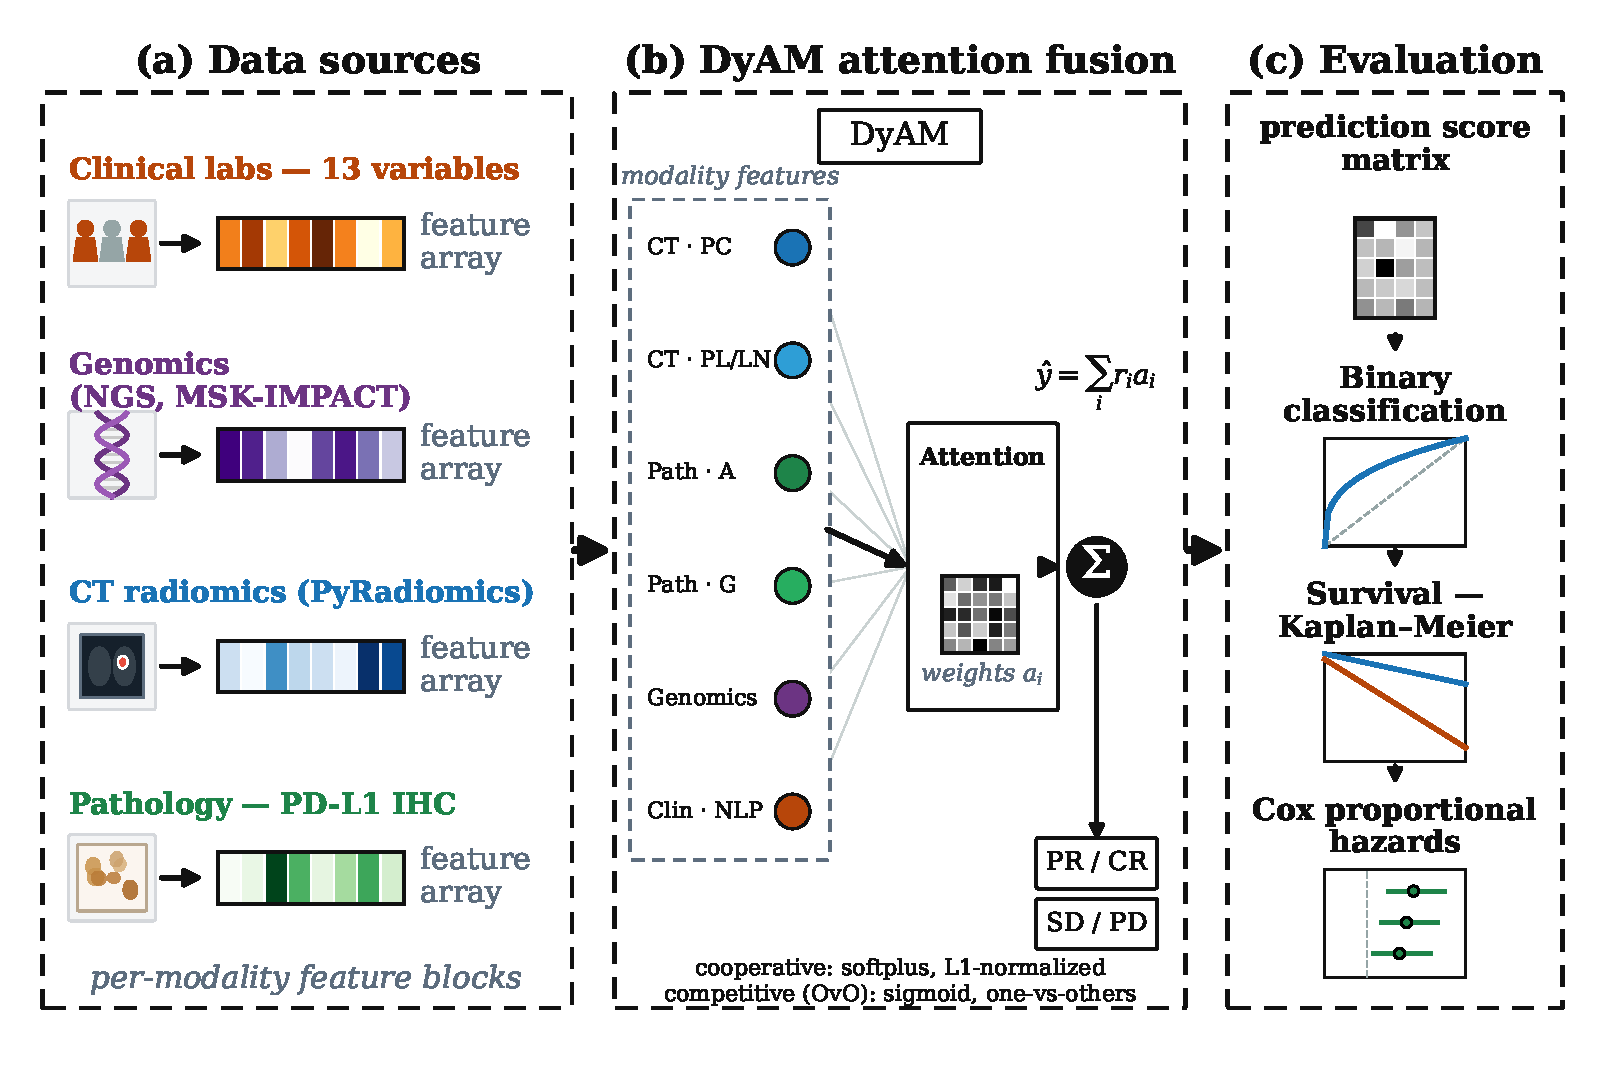
\includegraphics[width=\textwidth]{figures/fig1_overview_demo.pdf}
  \caption{Study overview. (A) The discovery cohort ($n = 247$) and two
    validation cohorts (radiomics-evaluable, $n = 50$; pathology-evaluable,
    $n = 71$) provide six data sources: CT radiomics (modelled separately
    per lesion site: PC, PL, LN), pathology image texture (IHC-A or IHC-G),
    tumour genomics, PD-L1~TPS, and structured clinical variables, giving up
    to seven input modalities per model. (B) The DyAM architecture computes a
    per-modality risk score and combines modalities using either cooperative
    (\texttt{AttentionMatrix}) or competitive one-vs-others
    (\texttt{AttentionMatrixOvO}) attention to produce a fused risk
    prediction $\hat{y}$. (C) Models are evaluated on both binary response
    classification (AUC-ROC with DeLong 95\% CI) and survival endpoints
    (Harrell's C-index, multivariate Cox hazard ratios, and Kaplan--Meier
    log-rank stratification).}
  \label{fig:overview}
\end{figure}

%% ═══════════════════════════════════════════════════════════════════════════
%% B2 — Data Modalities
%% ═══════════════════════════════════════════════════════════════════════════

\subsection{Data Modalities}
\label{sec:modalities}

Six data sources were assembled for each patient
(Table~\ref{tab:modalities}).
Because CT radiomics is modelled separately per lesion site (PC, PL, LN) and
the two pathology feature sets (IHC-A, IHC-G) are used as alternative arms
rather than jointly, a single model receives up to seven input modalities.
CT radiomics features were extracted from baseline scans using the MIRPON
pipeline \cite{Dercle2020} at 1.0~mm isotropic spacing with a window of
$[{-1350}, 250]$~HU, yielding 1{,}688 features per lesion type.
Lesions were categorised by anatomical site:
primary tumour (PC), pleural lesion (PL), and lymph node (LN).
Up to three lesions per site were included, ranked by volume.
Pathology features were derived from PD-L1 immunohistochemistry (IHC) slides:
\emph{IHC-A} comprised 18 pixel-intensity aggregation features
(area, mean intensity, percentiles), while
\emph{IHC-G} comprised 150 grey-level co-occurrence matrix (GLCM)
texture features across six aggregation levels \cite{Vanguri2022}.
Genomic features (11 variables) included tumour mutational burden (TMB) and
the status of eight driver mutations and amplifications derived from
FoundationOne~CDx next-generation sequencing (NGS).
The PD-L1 tumour proportion score (TPS) was obtained from clinical
pathology reports (range 0--100\%).
Clinical laboratory features comprised 13 variables:
age, smoking pack-years, Eastern Cooperative Oncology Group (ECOG)
performance status, serum albumin,
derived neutrophil-to-lymphocyte ratio (dNLR), initial tumour burden,
brain and liver metastasis status, line of therapy, combination therapy,
primary lung site, prior PD-L1 therapy, and adenocarcinoma histology.

For radiomics modalities, features with an intraclass correlation coefficient
(ICC) below 0.15 across test--retest perturbation scans were removed
(robustness filter), and features with a $z$-score exceeding 6 in any patient
were flagged as outliers and excluded.
All modalities except the NLP embedding (Section~\ref{sec:nlp}) were
standardised with \texttt{RobustScaler} (median centring, IQR scaling).
Missing modalities were handled via a binary indicator mask
$\mathbf{m} \in \{0,1\}^N$; masked modalities contribute zero attention and
zero risk to the fused prediction (Section~\ref{sec:model}).

\begin{table}[H]
\caption{Summary of data modalities used in this study.
  All feature counts are post-selection (after ICC and outlier filtering
  for radiomics).
  NLP, natural language processing; GLCM, grey-level co-occurrence matrix;
  IHC, immunohistochemistry; NGS, next-generation sequencing;
  TPS, tumour proportion score.}
\label{tab:modalities}
\small
\begin{tabular}{@{}p{2.3cm}p{2.7cm}p{1.2cm}p{4.1cm}@{}}
\toprule
\textbf{Modality} & \textbf{Source} & \textbf{Features} & \textbf{Clinical meaning} \\
\midrule
CT Radiomics (PC, PL, LN) & MIRPON pipeline & $\leq$1{,}688 & Tumour shape, size, and texture from baseline CT \\
Pathology IHC-A            & PD-L1 IHC slides & 18  & Pixel-intensity aggregation of PD-L1 expression \\
Pathology IHC-G            & PD-L1 IHC slides & 150 & GLCM texture of PD-L1 signal \\
Genomics                   & FoundationOne CDx & 11 & TMB + driver mutation/amplification status \\
PD-L1 TPS                  & Pathology report  & 1  & Tumour proportion score (0--100\%) \\
Clinical labs              & EHR               & 13 & Demographics, performance status, labs \\
\textbf{NLP embedding} (new) & \texttt{all-MiniLM-L6-v2} & 384 & Sentence embedding of clinical lab text \\
\textbf{NLP-PCA16} (new)   & PCA of NLP        & 16  & PCA-compressed NLP (approx.\ 94\% variance) \\
\bottomrule
\end{tabular}
\end{table}

%% ═══════════════════════════════════════════════════════════════════════════
%% B3 — NLP Clinical Embedding
%% ═══════════════════════════════════════════════════════════════════════════

\subsection{NLP Encoding of Tabular Clinical Features}
\label{sec:nlp}

Standard encoding of clinical variables as a 13-dimensional numeric vector
treats each feature independently and loses contextual relationships between
variables (e.g., an elderly patient with low albumin and ECOG~2 implies a
different prognosis than the same values in isolation).
To capture inter-feature context, we converted each patient's clinical
profile into an English-language sentence and extracted a dense semantic
embedding, as illustrated in Figure~\ref{fig:nlp_pipeline}.

\paragraph{Text prompt construction.}
For each patient, the 13 clinical variables were formatted into a structured
natural-language sentence, for example:
\textit{``The patient is a 69-year-old. Smoking history in pack-years is 48.0.
ECOG performance status is 1.0. Blood albumin concentration is 4.00.
Derived neutrophil-to-lymphocyte ratio (dNLR) is 2.40.
Initial tumor burden stands at 52.00.
The patient is diagnosed with adenocarcinoma at the lung site.
Metastatic status: without brain metastasis and without liver metastasis.
Currently undergoing therapy line 2, utilizing combination therapy.
The patient received prior PD-L1 immunotherapy.''}
Binary variables were expanded to descriptive phrases to exploit the
pretrained vocabulary of the encoder.
The full prompt template is provided in Supplementary Note~S1.

\paragraph{Sentence encoder.}
Prompts were encoded with
\texttt{sentence-transformers/all-MiniLM-L6-v2} \cite{Reimers2019,Wang2020MiniLM},
a 6-layer transformer distilled for semantic sentence similarity and
trained on over one billion sentence pairs.
Each patient was represented as a 384-dimensional L2-normalised vector.
No fine-tuning was performed; the model was applied in zero-shot transfer.
We compared this general-purpose encoder against the domain-specific
\texttt{Bio\_ClinicalBERT} \cite{Alsentzer2019};
the domain-specific model performed inferiorly
($\Delta\text{AUC} = -0.017$ versus MiniLM-L6-v2 in the IHC-A arm),
consistent with its design for masked language modelling
rather than sentence-similarity tasks (Supplementary Note~S2).

\paragraph{Dimensionality reduction.}
Principal component analysis (PCA) was applied to the 384-dimensional embeddings,
retaining the top 16 components ($\approx$94\% of variance explained;
Supplementary Figure~S1).
Both the raw 384-dimensional (\emph{NLP raw}) and PCA-compressed
16-dimensional (\emph{NLP-PCA16}) variants were evaluated.
Crucially, the NLP modality was passed to the model with the RobustScaler
disabled (\texttt{no\_scale=True}), as the embeddings are already L2-normalised
and scaling would distort the cosine-similarity geometry of the embedding space.

\begin{figure}[H]
  \centering
  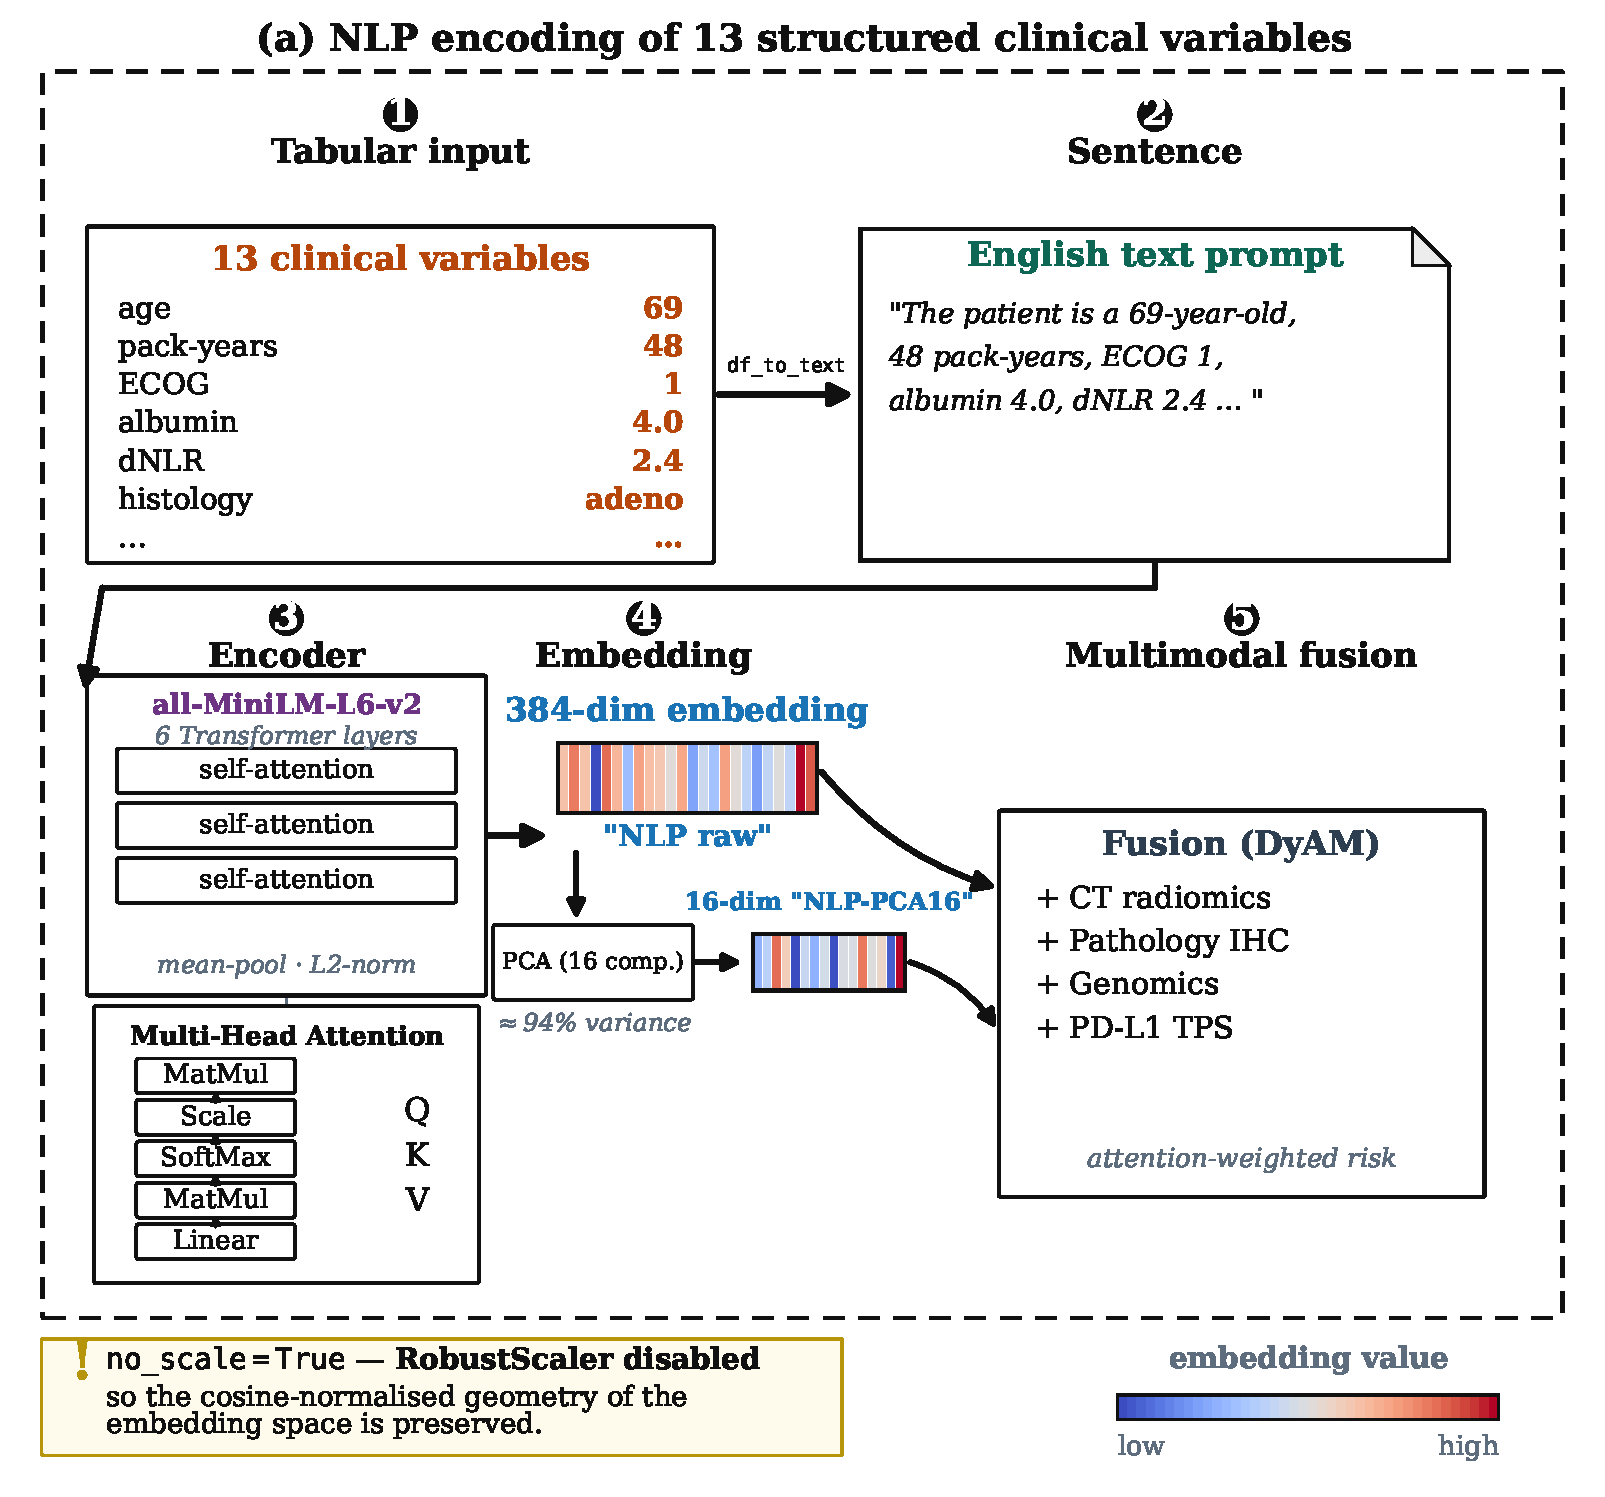
\includegraphics[width=\textwidth]{figures/fig2_nlp_pipeline_demo.pdf}
  \caption{NLP-based encoding of structured clinical features. Thirteen
    numeric clinical variables per patient are converted into a
    natural-language sentence describing the patient's clinical profile
    (example shown), which is then encoded into a 384-dimensional embedding
    using a pretrained sentence transformer (all-MiniLM-L6-v2). The
    384-dimensional embedding (``NLP raw'') is used directly, or further
    reduced to 16 dimensions via PCA (``NLP-PCA16'', retaining
    $\approx$94\% of variance) prior to fusion with other modalities.
    \texttt{no\_scale=True} is applied to NLP embeddings to preserve their
    cosine-normalised geometry.}
  \label{fig:nlp_pipeline}
\end{figure}

%% ═══════════════════════════════════════════════════════════════════════════
%% B4 — Model Architecture
%% ═══════════════════════════════════════════════════════════════════════════

\subsection{Model Architecture}
\label{sec:model}

\paragraph{Dynamic Attention Multimodal (DyAM) model.}
The base model, DyAM \cite{Vanguri2022}, fuses $N$ modalities through
per-modality risk scores and a learned attention mechanism, in the spirit of
attention-based architectures broadly \cite{Vaswani2017}.
Let $\mathbf{x}_i \in \mathbb{R}^{d_i}$ denote the feature vector of
modality~$i$ after optional RobustScaling.
A scalar risk score is computed as:
%
\begin{equation}
  r_i = \tanh\!\left(\mathbf{W}_{\mathrm{r},i}^{\top} \mathbf{x}_i\right),
  \label{eq:risk}
\end{equation}
%
where $\mathbf{W}_{\mathrm{r},i} \in \mathbb{R}^{d_i}$ are learnable weights.
An attention score is produced by an $N \times N$ grid of linear layers
with softplus activation, $\ell_2$-normalised by the modality vector norm:
%
\begin{equation}
  s_i = \frac{\mathrm{softplus}\!\left(\mathbf{W}_{\mathrm{a},ij}^{\top}
        \mathbf{x}_i\right)}{\left\|\mathbf{x}_i\right\|_2}.
  \label{eq:attn_s}
\end{equation}
%
Attention weights are obtained by L1 normalisation across modalities:
%
\begin{equation}
  a_i = \frac{s_i}{\displaystyle\sum_{j=1}^{N} s_j}.
  \label{eq:attn_a}
\end{equation}

\paragraph{OvO competitive attention.}
We propose an alternative attention mechanism inspired by
one-versus-others (OvO) classification \cite{Hastie1998},
in which each modality \emph{competes} against the mean score of
all remaining modalities rather than sharing a fixed budget.
The mean score of the $N-1$ competing modalities is:
%
\begin{equation}
  \mu_{-i} = \frac{1}{N-1} \sum_{j \neq i} s_j,
  \label{eq:ovo_mu}
\end{equation}
%
and the OvO attention score is:
%
\begin{equation}
  \mathrm{ovo}_i = \sigma\!\left(s_i - \mu_{-i}\right),
  \qquad \sigma(z) = (1+e^{-z})^{-1}.
  \label{eq:ovo}
\end{equation}
%
The sigmoid function yields an independent probability that modality~$i$
outperforms the others, rather than a jointly normalised score.
After applying the binary missingness mask $m_i \in \{0,1\}$, the weights
are L1-normalised: $a_i = \mathrm{ovo}_i \cdot m_i \big/
\sum_j \mathrm{ovo}_j \cdot m_j$.
The two attention mechanisms are contrasted schematically in
Figure~\ref{fig:attention_arch}.

\paragraph{Fused prediction and training.}
For both variants, the final risk prediction is:
%
\begin{equation}
  \hat{y} = \sum_{i=1}^{N} r_i \cdot a_i.
  \label{eq:output}
\end{equation}
%
\begin{figure}[H]
  \centering
  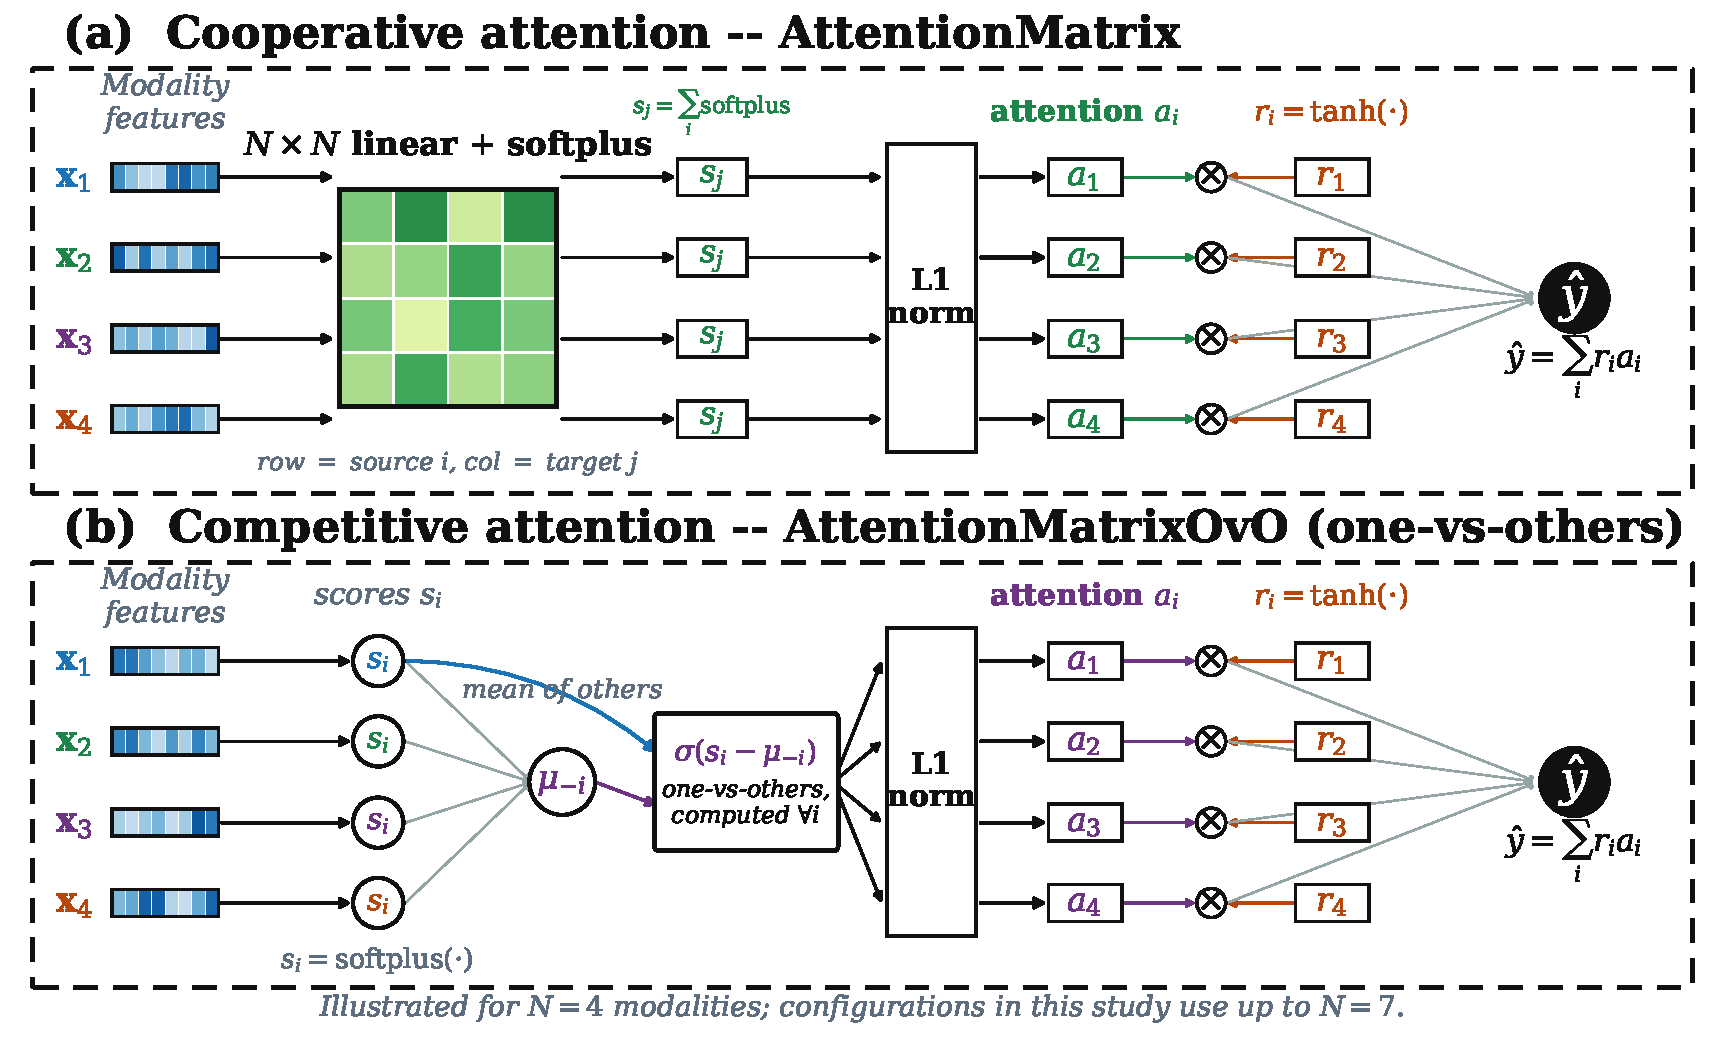
\includegraphics[width=\textwidth]{figures/fig_attention_arch_demo.pdf}
  \caption{Architecture of the two attention mechanisms. Both variants
    compute a per-modality risk score $r_i = \tanh(\mathbf{W}_{r,i}^{\top}
    \mathbf{x}_i)$ (Equation~\ref{eq:risk}) and produce the fused prediction
    $\hat{y} = \sum_i r_i a_i$ (Equation~\ref{eq:output}); they differ only in
    how the attention weights $a_i$ are obtained.
    (A)~\emph{Cooperative} attention (\texttt{AttentionMatrix}): an
    $N\times N$ grid of linear layers with softplus activation produces
    pairwise scores that are column-summed into $s_j$
    (Equation~\ref{eq:attn_s}) and L1-normalised so that the modalities
    share a fixed attention budget (Equation~\ref{eq:attn_a}).
    (B)~\emph{Competitive} one-vs-others attention
    (\texttt{AttentionMatrixOvO}): each modality produces a single score
    $s_i$ that is compared against the mean score of the remaining
    modalities $\mu_{-i}$ through a sigmoid, $\sigma(s_i - \mu_{-i})$
    (Equations~\ref{eq:ovo_mu}--\ref{eq:ovo}), yielding an independent
    competitive weight before L1 normalisation.
    Heatmap bars denote modality feature vectors; the diagram is drawn for
    $N = 4$ modalities for clarity.}
  \label{fig:attention_arch}
\end{figure}

The model was trained with binary cross-entropy loss
(\texttt{BCEWithLogitsLoss}) with automatic inverse-frequency class
weighting to address the $\approx$1:3 class imbalance,
$\ell_1$ regularisation on attention weights ($\alpha = 1.0$),
and $\ell_2$ weight decay ($\beta = 1.0$).
The Adam optimiser was used with a learning rate of 0.01 for 125 epochs.
All experiments used 10-fold stratified cross-validation on the
discovery cohort; predictions were pooled across held-out folds for
AUC computation.

%% ═══════════════════════════════════════════════════════════════════════════
%% B5 — Statistical Analysis
%% ═══════════════════════════════════════════════════════════════════════════

\subsection{Statistical Analysis and Evaluation}
\label{sec:stats}

\paragraph{Discriminative performance.}
Area under the receiver operating characteristic curve (AUC-ROC) was
computed on pooled out-of-fold predictions from 10-fold cross-validation.
Ninety-five percent confidence intervals (CIs) were estimated using the
DeLong structural components method \cite{DeLong1988}.
Two models were considered statistically significantly different when their
95\% CIs did not overlap, consistent with standard practice in oncology
imaging studies.

\paragraph{Survival analysis.}
Harrell's concordance index (C-index) \cite{Harrell1996} was computed from
pooled out-of-fold risk scores against PFS.
Bootstrap 95\% CIs were derived from 1{,}000 resamples with replacement.
For pairwise comparisons, per-fold C-indices (10 values) were compared with
a two-sided Wilcoxon signed-rank test ($\alpha = 0.05$).
Time-dependent AUC was computed at 6, 12, and 18~months using the
cumulative/dynamic estimator \cite{Harrell1996}.
Multivariate Cox proportional hazards regression was fitted with the
DyAM risk score as the primary predictor, adjusted for five clinical
covariates: age, ECOG performance status, serum albumin, dNLR, and
liver metastasis status.
Hazard ratios (HRs) are reported with 95\% CIs and Wald $p$-values.
Model calibration was assessed via the Integrated Brier Score (IBS);
values below 0.25 indicate better-than-random calibration.

\paragraph{Kaplan--Meier survival stratification.}
Patients were dichotomised at risk score~$= 0$, and PFS curves for the
two groups were compared with the log-rank test.
A threshold of $\chi^2 > 7.88$ ($p < 0.005$) was applied as the
significance criterion, consistent with oncology reporting standards.

\paragraph{Software.}
All analyses were performed in Python~3.10 using PyTorch~2.0 (model training),
\texttt{lifelines}~0.27 (Kaplan--Meier, Cox regression, C-index),
\texttt{scikit-survival}~0.21 (time-dependent AUC, Brier score),
and \texttt{scipy}~1.11 (Wilcoxon test).
